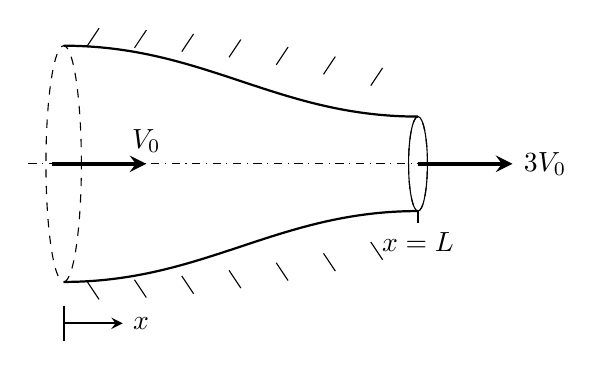
\begin{tikzpicture}[>=stealth, scale=1.5]
    % Nozzle walls
    \draw[thick] (0,1) to[out=0, in=180] (3,0.4);
    \draw[thick] (0,-1) to[out=0, in=180] (3,-0.4);
    
    % Hatching for walls
    \foreach \x in {0.2,0.6,...,2.8} {
        \draw (\x, {1 - 0.05*\x*\x}) -- (\x+0.1, {1.15 - 0.05*\x*\x});
        \draw (\x, {-1 + 0.05*\x*\x}) -- (\x+0.1, {-1.15 + 0.05*\x*\x});
    }

    % Entrance boundary (Dashed around the nozzle)
    \draw[dashed] (0,0) ellipse (0.15 and 1);
    
    % Exit boundary (Dashed around the nozzle)
    \draw[dashed] (3,0) ellipse (0.08 and 0.4);
    \draw (3,0) ellipse (0.08 and 0.4); % Solid front of the exit

    % Centerline (Only within the flow region)
    \draw[dashdotted] (-0.3,0) -- (3.5,0);

    % Velocity Vectors
    \draw[->, ultra thick] (-0.1,0) -- (0.7,0) node[above] {$V_0$};
    \draw[->, ultra thick] (3,0) -- (3.8,0) node[right] {$3V_0$};

    % Coordinate/Position Labels
    \draw[thick] (0,-1.2) -- (0,-1.5);
    \draw[->, thick] (0,-1.35) -- (0.5,-1.35) node[right] {$x$};
    \node[below] at (3,-0.5) {$x=L$};
    \draw[thick] (3,-0.4) -- (3,-0.5);
\end{tikzpicture}
